\documentclass[../mainfile.tex]{subfiles}

\begin{document}
\section{Donsker's Theorem}
We will now briefly outline two proofs of Donsker's theorem.
\subsection{Formulation of the theorem}
\begin{itemize}
\item We work on the metric space $(E,d)$ where $E= \mathcal{C}([0,1] \to \mathbb{R})$ denotes the space of continuous function from $[0,1]$ to $\mathbb{R}$, endowed with the metric $d(f,g)= \max_{[0,1]} |f-g|$. 
\item The Wiener measure is then the law of $(B_t, t \in [0,1])$ viewed as an element of said metric space $(E,d)$. 
\item On the same metric space we consider the \textit{"interpolated, rescaled random walk"} defined as follows:
\begin{enumerate}
\item We start with a standard random walk $S_n:=X_1 + \dots + X_n$, i.e. $S_0:=0$ and the $X_i$ are i.i.d. coin flips. 
\item We extend this into a continuous function $(S_t, t \geq 0)$ by linearly interpolating the previous sequence on each interval $[n,n+1]$.
\item For each $\epsilon >0$, we define the rescaled Random Walk (notice that we both scale time and our "height") by
\begin{align*}
S_t^{(\epsilon)}:= \epsilon S_{\epsilon^{-2}t}.
\end{align*}
We then look at $(S_t^{(\epsilon)}, t \leq 1)$ as a random element in $(E,d)$. 
\end{enumerate}
\end{itemize}
\begin{thm}[Donsker's invariance theorem] The law of $(S_t^{( \epsilon)}, t \leq 1)$ (viewed as a measure on $(E,d)$) converges weakly as $\epsilon \to 0$ to the law of $B$ (viewed as a law in $(E,d)$ i.e. Wiener measure).
\end{thm}
\begin{rem} This means that for all continuous functions $F: (E,d) \to \mathbb{R}$ we have 
\begin{align*}
\mathbb{E}(F(S^{(\epsilon)})) \overset{\epsilon \to 0}\longrightarrow \mathbb{E}(F(B))
\end{align*}
Also it is worth to mention that if we work with $F(f):=f(1)$ (which is continuous with respect to $d$) then this can be used to deduce the regular Central Limit Theorem (substitute $u= \frac{1}{\epsilon^2}$ so as $\epsilon \to 0$ we have $u \to \infty$ and $\epsilon = \frac{1}{\sqrt{u}}$) 
\end{rem}
\newpage
\subsection{Warm-up: Doob's inequality for discrete martingales}
A general useful tool to have information about \textit{"regularity of entire trajectories"} is Doob's inequality for discrete martingales. We provide here a quick recap of the various results. 
\\\\
We write 
\begin{align*}
M_n^*:= \max_{0 \leq j \leq n} |M_j|.
\end{align*}
Trivially we have $M_n^* \geq |M_n|$. The purpose of Doob's inequalities is to conversely provide upper bounds for $M_n^*$ in terms of $|M_n|:$
\begin{itemize}
\item \textbf{Doob's maximal inequality:} If $(M_n)_{n \geq 0}$ is a martingale with respect to the filtration $( \mathcal{F}_n)_{n \geq 0}$ such that $M_0=0$ almost surely, then for all $\lambda >0$ and all $N \geq 0 $: 
\begin{align*}
\lambda \mathbb{P}( M_N^* \geq \lambda) \leq \mathbb{E}(|M_N|1_{M_N^* \geq \lambda}) \leq \mathbb{E}(|M_N|).
\end{align*}
\item \textbf{Doob's $L^2$ inequality:} If furthermore the random variables $M_n$ are in $L^2$, then one always has
\begin{align*}
\mathbb{E}((M_N^*)^2) \leq 4 \mathbb{E}(M_N^2). 
\end{align*}
This is very useful as it allows to control the whole trajectory of $M$ until time $N$ via the law of $M_N$ only. 
\item \textbf{Doob's $L^p$ inequality:} Similarly, if the random variables $M_n$ are in $L^p$ for some $p >1$, then
\begin{align*}
\mathbb{E}((M_N^*)^p) \leq (p/(p-1))^p \mathbb{E}(|M_N|^p). 
\end{align*}
\end{itemize} 
\newpage
\subsection{Proof via coupling}
\begin{proof}[Proof of Donsker's theorem] First we roughly describe the idea of the proof. We start with a Brownian motion $(B_t)_{t \geq 0}$. Then we define deterministically (as a function of $B$) for each given $\epsilon >0$ a rescaled Random Walk $S^{(\epsilon)}$ that is going to be very close to $B$.\\
\\
Let us define for each $\epsilon >0$ a sequence of $T_n^\epsilon$ of stopping times by: $T_0^\epsilon =0$ 
\begin{align*}
T_1^\epsilon &= \inf \{ t >0 : |B_t| = \epsilon \} \\
T_n^\epsilon& = \min \{ t> T_{n-1}^\epsilon : |B_t-B_{T_{n-1}^\epsilon}| = \epsilon \}. 
\end{align*}
\begin{figure}[hbtp]
\centering
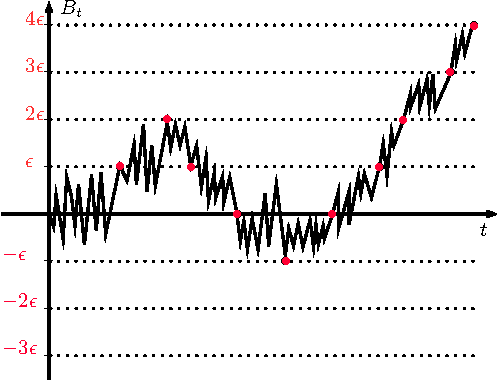
\includegraphics[scale=1]{donsker1.pdf}
\caption{The stopping times $T_n^\epsilon$ indicated with red dots. }
\end{figure}
\\
We then define 
\begin{align*}
S_n^\epsilon := \frac{B_{T_n^\epsilon}}{\epsilon},
\end{align*}
we notice that in our realisation as in the figure above we have $S_1^\epsilon
=1$ whereas $S_5^\epsilon = -1$. We see that $(S_n^\epsilon)_{n \geq 0}$ is a simple random walk. We will later discuss this in more detail. \\
\\
Next we define $(S_t^\epsilon)_{t \geq 0}$ by linear interpolation on each $[n,n+1]$. Then the rescaled random walk 
\begin{align*}
(S_t^{( \epsilon)} = \epsilon S_{ \epsilon^{-2} t}^\epsilon )_{t \geq 0}. 
\end{align*}
\newpage
\begin{figure}[hbtp]
\centering
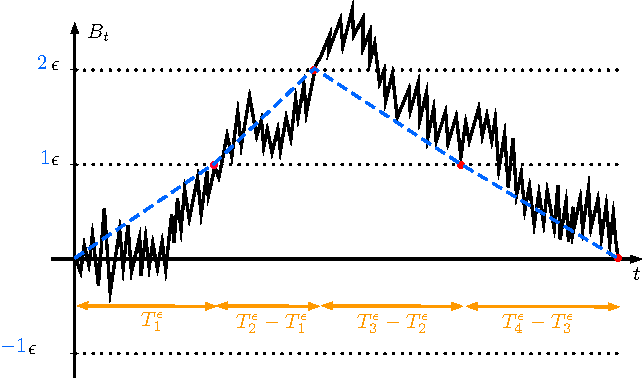
\includegraphics[scale=1]{donsker2.pdf}
\caption{We notice ($\approx$blue line) that $S_1^\epsilon = 1$, $S_2^\epsilon = 2$, $S_3^\epsilon =1$, $S_4^\epsilon = 0$. So our increments are $\pm 1$. }
\end{figure}
\begin{figure}[hbtp]
\centering
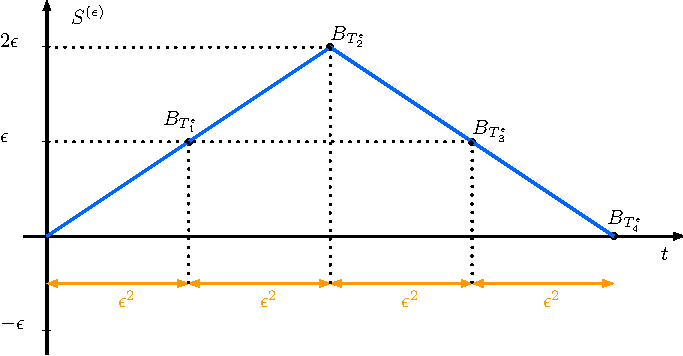
\includegraphics[scale=.9]{donsker3.pdf}
\caption{The graph of $S^{( \epsilon)}$, notice that for each $t=n \epsilon^2$, the value of $S^{( \epsilon)}$ is exactly $B_{T_n^\epsilon}$. }
\end{figure}
We observe:
\begin{itemize}
\item $(T_{n+1}^\epsilon-T_n^\epsilon)_{n \geq 0}$ is a sequence of i.i.d. RV (strong Markov property).
\item By scaling: The law of $\tau_n:=\displaystyle \frac{T_{n+1}^\epsilon-T_n^\epsilon}{\epsilon^2}$ does not depend on $\epsilon$. 
\item $\mathbb{E}(\tau_1)=1$ (using $B_t^2-t$ is martingale) $\rightsquigarrow \mathbb{E}(T_n^\epsilon)=n \epsilon^2$ (by independence).
\item The random variables $(X_n^\epsilon := \epsilon^{-1}(B_{T_n^\epsilon}-B_{T_{n-1}^\epsilon})$ are i.i.d. coin flips. 
\end{itemize}
\newpage
\textbf{Goal:} We want to show that $(S_s^{(\epsilon)})_{ s \leq 1}$ converges in law/weakly in $(E,d)$ to $(B_s, s \leq 1)$ as $\epsilon \to 0$. \\
\\
We will show a stronger statement,  i.e. that $S_s^{( \epsilon)}$ is actually very close to $B$ in the sup norm. More precisely, we want to show that
\begin{align*}
\forall \eta > 0, \forall \alpha > 0, \exists \epsilon_0 : \forall \epsilon \text{ with } \epsilon < \epsilon_0 , \ \mathbb{P}( \sup_{ s \in [0,1]} |B_s-S_s^{( \epsilon)} | > \alpha) < \eta. \tag{*}
\end{align*}
In order to establish (*) we will derive another inequality: For each $\epsilon >0$ and each $s \leq 1$, let us define $t_\epsilon(s)$ to be the largest multiple of $\epsilon^2$ such that $t_\epsilon(s) \leq s$, we then get:
\begin{align*}
\sup_{ s \in [0,1]} |B_s-S_s^{( \epsilon)}| &=\sup_{s \in [0,1]} |B_s-B_{t_\epsilon(s)} +B_{t_\epsilon(s)} - S_{t_\epsilon(s)}^{(\epsilon)}+S_{t_\epsilon(s)}^{(\epsilon)}-S_s^{(\epsilon)}| \\
& \leq \sup_{s \in [0,1]} |B_s-B_{t_\epsilon(s)}| + \sup_{s \leq 1} | S_s^{ (\epsilon)} -S_{t_\epsilon(s)}^{( \epsilon)}|+ \sup_{s \leq 1}|B_{t_\epsilon(s)}-S_{t_\epsilon(s)}^{( \epsilon)}| \\
& \leq  \sup_{s \in [0,1]} |B_s-B_{t_\epsilon(s)}| + \sup_{s \leq 1} | S_s^{ (\epsilon)} -S_{t_\epsilon(s)}^{( \epsilon)}|+ \max_{j \leq \epsilon^{- 2}} |B_{j \epsilon^2}-S_{j \epsilon^2}^{(\epsilon)}| \\
&=   \sup_{s \in [0,1]} |B_s-B_{t_\epsilon(s)}| + \sup_{s \leq 1} | S_s^{ (\epsilon)} -S_{t_\epsilon(s)}^{( \epsilon)}|+ \max_{j \leq \epsilon^{- 2}} |B_{j \epsilon^2}-B_{T_j^\epsilon}|
\end{align*}
We immediately notice that by definition we have
\begin{align*}
|S_{t_\epsilon(s)}^{( \epsilon)}-S_s^{(\epsilon)}| \leq \epsilon.
\end{align*}
So we will choose $\epsilon_0 \leq \alpha/4$ such that finally we want to get an upper bound of $\sup |B_s-S_s^{( \epsilon)}| \leq  3\alpha /4$.
\\\\
On the other hand, we know that almost surely $B$ is continuous on $[0,2]$, so that almost surely, for all given $\alpha >0$, there exists a (random) $\delta >0$ such that for all $s,t \leq 2$ with $|s-t| \leq \delta$ we have  
\begin{align*}
|B_s-B_t| \leq \frac{\alpha}{4}. \tag{**}
\end{align*}
For all $\eta >0$, we can always choose $\delta_0=\delta_0( \alpha, \eta)$ small enough, such that the random $\delta>0$ above is larger than $\delta_0$ with probability at least $1-\eta/4$.  \\\\
Hence, on this event of probability at least $1- \eta/4$, by (**) in order to ensure that
\begin{align*}
 \sup_{s \in [0,1]} |B_s-B_{t_\epsilon(s)}| + \max_{j \leq \epsilon^{- 2}} |B_{j \epsilon^2}-B_{T_j^\epsilon}| \leq \frac{\alpha}{2} 
\end{align*}
it is enough to force that
\begin{align*}
\sup_{ s \leq 1} |s-t_\epsilon(s)| \leq \delta_0 \text{ and } \max_{j \leq \epsilon^{-2}} |j \epsilon^2 -T_j^\epsilon| \leq \delta_0.
\end{align*}
\newpage
We first notice that $|s-t_\epsilon(s)| \leq \epsilon^2$, so we choose $\epsilon_0^2 \leq \delta_0$. \\
\\
In order to establish the second bound, we consider 
\begin{align*}
M_n:= T_n^\epsilon- \mathbb{E}(T_n^\epsilon)= (T_1^\epsilon- \mathbb{E}(T_1^\epsilon))+ ( T_2^\epsilon-T_1^\epsilon- \mathbb{E}(T_1^\epsilon))+ \dots + ( T_n^\epsilon-T_{n-1}^\epsilon - \mathbb{E}(T_1^\epsilon))
\end{align*}
Since $M_n$ can be written as the sum of i.i.d. Random Variables with mean $0$ we can conclude that $(M_n)_{n \geq 0}$ is a martingale. Moreover it has finite bounded variance, in particular we can use Doob's $L^2$-inequality (note that $M_n= T_n^\epsilon- n \epsilon^2)$. We denote by $u_\epsilon$ the integer part of $\epsilon^{-2}$: 
\begin{align*}
\mathbb{E}( ( \max_{j \leq u_\epsilon} (T_j^\epsilon-j \epsilon^2)^2)& \leq 4 \mathbb{E}((T_{u_\epsilon}^\epsilon-u_\epsilon \epsilon^2)^2) = 4 \text{var}(T_{u_\epsilon}^\epsilon) \\
&=4 \text{var}( T_1^\epsilon + (T_2^\epsilon-T_1^\epsilon) + \dots + (T_{u_\epsilon}^\epsilon-T_{u_\epsilon-1}^\epsilon)) \\
&= 4 u_\epsilon\text{var}(T_1^\epsilon) \leq 4 \epsilon^{-2} \text{var}(T_1^\epsilon) \leq 4 \epsilon^{-2} \epsilon^4\text{var}(T_1^1) \\
&= 4 \epsilon^2 \text{var}(T_1^1)
\end{align*}
where the last inequality is just due to scaling. Hence, by Markov's inequality we obtain,
\begin{align*}
\mathbb{P}( \max_{j \leq u_\epsilon} |T_j^\epsilon-j \epsilon^2| \geq \sqrt{\epsilon})  \leq \epsilon ^{-1} \mathbb{E}( (\max_{j \leq u_\epsilon} (T_j^\epsilon-j \epsilon^2))^2) \leq 4 \epsilon \text{var}(T_1^1) \overset{!}<\frac{\eta}{4},
\end{align*}
hence, if we choose $\epsilon_0 \leq \delta_0^2 $ and $\epsilon_0 \leq \eta/(16 \text{var}(T_1^1))$, we get as soon as $\epsilon \leq \epsilon_0$, with probability at least $1-\eta/4$, 
\begin{align*}
\max_{j \leq u_\epsilon} |T_j^\epsilon-j \epsilon^2| \leq \delta_0. 
\end{align*}
In conclusion, for all $\alpha>0$ and $\eta>0$, if we choose \\ $\epsilon_0 \leq \min( \delta_0^2, \eta/(16 \text{var}(T_1^1)), \sqrt{\delta_0}, \alpha/4)$ for $\delta_0=\delta_0( \eta, \alpha)$, we get indeed that for all $\epsilon \leq \epsilon_0,$ 
\begin{align*}
\mathbb{P} ( \sup_{s \in [0,1]} |B_s-S_s^{( \epsilon)} | > \alpha ) < \eta,
\end{align*}
which concludes the proof of Donsker's theorem. 
\end{proof}
\begin{rem} We stress the fact, that the approach we choose to prove Donsker's theorem here was that of a natural embedding of a random walk within a Brownian motion. This is an idea that will resurface again when we will study general continuous martingales.
\end{rem}
\newpage
\subsubsection{Some consequences}
Donsker's theorem allows for instance to derive results for the limiting distribution of \textit{continuous functionals} of simple random walks in terms of the corresponding continuous functionals of Brownian motion. More precisely, if $F$ is a continuous function from the space of continuous function on $[0,1]$ (endowed with the sup norm) onto some other metric space, then Donsker's theorem shows that the law of $F((S_t^{( \epsilon)}, t \in [0,1]))$ converges weakly to that of $F((B_t,t \in [0,1]))$ as $\epsilon \to 0$. 
\begin{exmp}Let $f^*$ denote the function that associates to a continuous function $f$ its maximum on $[0,1]$, i.e. $f^* : (\mathcal{C},d) \to \mathbb{R}$ given by
\begin{align*}
f^*(f):= \max_{t \in [0,1]} f(t).
\end{align*}
By Donsker's theorem we get that $\max_{[0,1]} S^{( \epsilon)}$ converges to the law of $\max_{[0,1]} B$ as $\epsilon \to 0$. 
\end{exmp}
\begin{exmp} We define for each $f \in \mathcal{C}$: \begin{align*}
f^*(t)&:= \sup_{s \leq t} f(s) \\
f^\#(t)&:= \inf_{s \leq t} f(s)
\end{align*}
then $f^*,f^\#$ are again in $\mathcal{C}$, we then define 
\begin{align*}
F: \begin{cases} E & \longrightarrow E^3 \\
f & \longmapsto (f,f^*,f^\#) \end{cases}
\end{align*}
Donsker's theorem then implies that weak convergence of the triples
\begin{align*}
(S^{( \epsilon)}, (S^{( \epsilon)})^*, (S^{( \epsilon)})^\#) \overset{\epsilon \to 0}\implies (B,B^*,B^\#)
\end{align*}
\end{exmp}
It will be shown in the exercise sheet that one can use Donsker's theorem to prove the following result:
\begin{prop}[Paul Lévy - one of his many results on BM] \ \\ Let $(B_t, t \geq 0)$ be a one dimensional Brownian motion started from the origin and define $\overline{B}_t := \max_{[0,t]} B$. Then the process $(\overline{B}_t-B_t, t \geq 0)$ has the same law as the process $( |B_t|, t \geq 0)$. 
\end{prop}
\begin{rem} Recall that it is possible to see as a rather consequence of the reflection principle that for a \textit{fixed} time $t$, the law of $\overline{B}_t-B_t$ is the same as that of $|B_t|$. The present statement is much stronger because it shows the identity in the law of the entire processes. This result will be derived (with two approaches, one using Donsker's thm) in the exercise sheet 6.
\end{rem}
\newpage
\subsection{Proof via compactness arguments}
We briefly discuss an alternate way how once could prove Donsker's theorem. We will only quickly browse through the arguments here, since the ideas presented wont be used again later on. 
\\\\
We start with a general fact:
\begin{itemize}
\item If $(P_n)_{n \in \mathbb{N}}$ is a sequence of probability measures on a compact metric space ($K,d)$, then there exists a subsequence $(n_k)$ such that $P_{n_k}$ converges weakly to some probability measure $P$ on $K$.
\end{itemize}
This result (and its proof) is a rather direct extension of the usual diagonal extraction trick. 
\begin{defn} If $(P_n)_{n \in \mathbb{N}}$ is a sequence of probability measures in a separable metric space, then the sequence is said to be \textbf{tight} if for all $\epsilon >0$ there exists a compact set $K$, such that for all $n \in \mathbb{N}$ 
\begin{align*}
P_n(K) \geq 1- \epsilon. 
\end{align*}
\end{defn}
\begin{thm}[Prokhorov Theorem 1/2] If $(P_n)_{n \in \mathbb{N}}$ is a tight sequence of probability measures in a separable metric space $(E,d)$, then there exists a subsequence $(n_k)$ such that $P_{n_k}$ converges weakly to some probability measure $\mathbb{P}$ on $E$. 
\end{thm}
We will apply this as follows in order to conclude Donsker's theorem:
\begin{itemize}
\item We consider $(E,d)$ the metric space of continuous functions on $[0,1]$ to $\mathbb{R}$ endowed with the sup norm, which is indeed a separable metric space. 
\item Let $(P_n)_{n \in \mathbb{N}}$ be a sequence of probability measures given by the law of $S^{( \epsilon_n)}$ for some $\epsilon_n \to 0$ as $n \to \infty$. 
\item We ask if the sequence $(P_n)_{n \in \mathbb{N}}$ is tight? 
\end{itemize} 
If we can prove that $(P_n)_{n \in \mathbb{N}}$ is tight, then by Prokhorov's theorem there exists $n_k$ and a probability measure $\mathbb{P}$ on $(E,d)$ such that $P_{n_k} \implies \mathbb{P}$. In particular we have for all $0\leq t_1< \dots < t_p \leq 1$, the function
\begin{align*}
F: \begin{cases} (E,d) & \longrightarrow \mathbb{R}^p \\
f & \longmapsto (f(t_1), \dots , f(t_p))
 \end{cases}
\end{align*}
then $F$ is continuous and thus we have $F(S^{( \epsilon_{n_k})}) \implies F(f)$ where $f \sim \mathbb{P}$. But we also know by the usual CLT that $(S^{( \epsilon_{n_k})}(t_1), \dots , S^{( \epsilon_{n_k})}(t_p)) \implies (B_{t_1}, \dots , B_{t_p})$ where $B$ is a BM, we conclude that $\mathbb{P}$  must be the Wiener measure. 
\newpage
So, in order to conclude Donsker's invariance theorem with this approach, it suffices to show that $(P_n)_{n \in \mathbb{N}}$ is indeed a tight sequence. This is part of the exercise sheet 7. \\
\\
For this, we can for instance use the following compact subset of $E$: For each $M>0$ let us define
\begin{align*}
K_M:= \{ f \in E : f(0)=0 \text{ and } \forall s,t \in [0,1], \ |f(t)-f(s)| \leq M |t-s|^{1/8}\}.
\end{align*}
The set $K_M$ is then a compact subset of $E$ by standard Arzelà-Ascoli considerations. On the other hand, it is not very difficult to show that for every $\eta >0$, there exists $M_\eta$ such that for all $\epsilon \leq 1$ we have  
\begin{align*}
\mathbb{P}(S^{( \epsilon)} \in K_M) \geq 1 - \eta. 
\end{align*}
which shows that the sequence $P_n$ is tight and provides another proof of Donsker's invariance principle. 
\end{document}